\documentclass[DIV=15]{scrartcl}
\usepackage{amsmath}
\usepackage{amssymb}
\usepackage{amsfonts}
\usepackage{bbm}
\usepackage{graphicx}
\usepackage{wrapfig} 
\graphicspath{{img/}}
\usepackage[ngerman]{babel}
\usepackage[T1]{fontenc}
\usepackage{comfortaa}
\renewcommand{\sfdefault}{comfortaa}
\title{Einführung in die Theoretische Informatik}
\author{Felix Ichters, Lukas Dzielski\thanks{Universität Heidelberg}}
\date{Sommersemester 2023}

%Titelblatt
\begin{document}
\maketitle
\rule{467.1pt}{0.4pt}

\begin{abstract}
\begin{flushright}
    \textit{Begleitmaterial mit den wichtigsten Definitionen und Aufgabenstellungen zur Vorlesung 'Einführung in die Theoretische Informatik'.}
\end{flushright}    
\end{abstract}
\bigskip\bigskip
\begin{center}
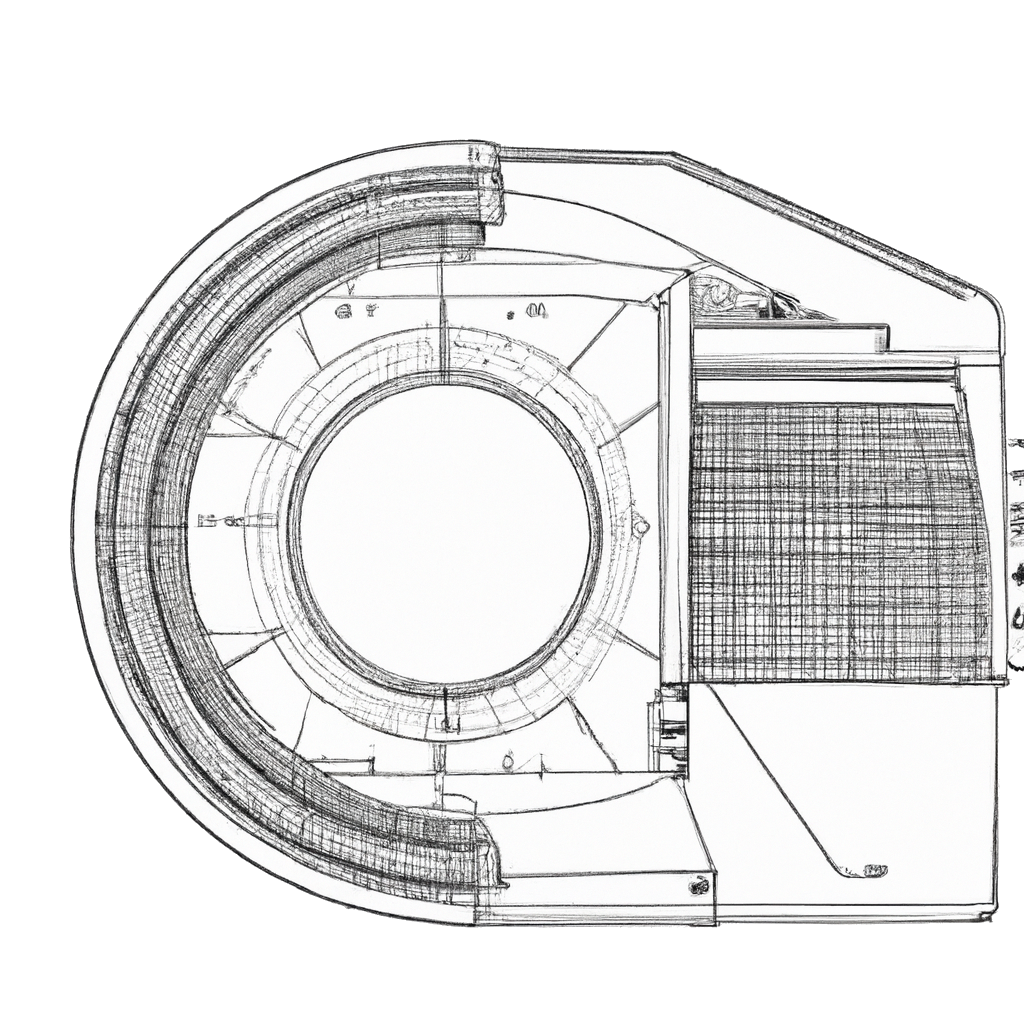
\includegraphics[width=0.5\textwidth]{dall2.png}    
\end{center}

%Inhaltsverzeichnis
\newpage
\tableofcontents
\newpage
\section{Notationen}
%\rule{467.1pt}{0.4pt}
\begin{itemize}
    \item Für \(n\in\mathbb{N}_0\), sei \([n]=\{1,\dots,n\}\) und \([n]_0=\{0,1,\dots,n\}\).
    \item Für eine Menge A und \(n\in\mathbb{N}\) ist \(A^n=\{(a_1,\dots,a_n):a_1,\dots,a_n\in A\}\).
    \item Für \(n\in\mathbb{N}\) ist eine n-äre partielle Funktion \(\varphi:A^n\rightsquigarrow B\) eine Funktion
    mit \(dom(\varphi)\subseteq A^n\) und \(Im(\varphi)\subseteq B\).
    Für \(a_1,\dots,a_n\in A\) bedeutet \(\varphi(a_1,\dots,a_n)\downarrow\), dass \(a_1,\dots,a_n\in dom(\varphi)\) gilt und 
    \(\varphi(a_1,\dots,a_n)\uparrow\) beduetet, dass \((a_1,\dots,a_n)\notin dom(\varphi)\).
    Die partielle Funktion \(\varphi\) ist total, wenn \(dom(\varphi)=A^n\) gilt.
    \item Eine lineare Ordnung auch totale Ordnung, auf einer Menge A ist eine Relation \(\leq\subseteq A^2\), so dass 
    die folgenden Eigenschaften erfüllt sind
        \subitem \(a\leq a\) \(\forall a\in A\) (Reflexivität)
        \subitem \(a\leq b\wedge b\leq a\Rightarrow a=b\) \(\forall a,b\in A\) (Antisymmetrie)
        \subitem \(a\leq b,b\leq c\Rightarrow a\leq c\) \(\forall a,b,c\in A\) (Transitivität)
        \subitem \(a\leq b\vee b\leq a\) \(\forall a,b\in A\) (Totalität)
\end{itemize}
\newpage
\part{Definitionen}
\rule{467.1pt}{0.4pt}
%Inhalt
\section{Grundlagen}
    \subsection{Alphabet}
        Ein Alphabet ist eine nichtleere Menge \(\Sigma\),die Elemente heißen Symbole.
    \subsection{Wörter}
        Ein Wort über einem Alphabet \(\Sigma\) ist eine endliche Folge von Symbolen aus \(\Sigma\).\\
        Für \(i\in[|w|]\) bezeichnet \(w(i)\) das i-te Element von w und für Symbole \(a_1,\dots,a_n\in \Sigma\)
        bezeichnet \(a_1,a_2,\dots,a_n\) das Wort w der Länge n mit \(w(i)=a_i\) \(\forall i\in [n]\).
    \subsection{Sprache}
        Eine Sprache ist eine Menge von Wörtern über einem gemeinsamen Alphabet \(\Sigma\).
    \subsection{\(\Sigma^*\)}
        Die Menge aller Wörter über \(\Sigma\) wird mit \(\Sigma^*\) bezeichnet.\\
        Für \(n\in\mathbb{N}_0\) setzen wir
        \[\Sigma^{\leq n}:=\{w\in\Sigma^*:|w|\leq n\}\]
        \[\Sigma^{=n}:=\{w\in\Sigma^*:|w|=n\}\]
        \[\Sigma^{\geq n}:=\{w\in\Sigma^*:|w|\geq n\}\]
        \[\Sigma^{+}:=\Sigma^{\geq 1}\]
    \subsection{Verkettung}
        Für Wörter \(w_1,w_2\) ist die Verkettung \(w_1w_2\) ist definiert durch 
        \[w_1w_2:=w_1(1)\dots w_1(|w_1|)w_2(1)\dots w_2(|w_2|).\]
        Für Sprachen \(L_1,L_2\) sei \(L_1L_2\) definiert durch 
        \[L_1L_2:=\{w_1w_2:w_1\in L_1, w_2\in L_2\}\]
    \subsection{Präfix, Infix, Suffix}
        Seien u,v Wörter 
        \begin{itemize}
            \item u ist Präfix von v, kurz \(u\sqsubseteq v\), falls es ein Wort w gibt, sodass uw=v 
            \item u ist Infix von v, falls es Wörter \(w_1,w_2\) gibt, sodass \(v=w_1uw_2\)
            \item u ist Suffix von v, falls es ein Wort w gibt, sodass v=wu
        \end{itemize}
    \subsection{Homomorphismus}
        Für Sprachen \(L,M\) heißt eine Funktion \(\varphi:L\to M\) 
        Homomorphismus von Sprachen, wenn gilt: \[\varphi(uv) = \varphi(u)\varphi(v)\]
    \subsection{Längenlexikographische Ordnungen}
        Es gilt \(u \leq_{llex} v\) wenn eine der folgenden Bedingungen erfüllt ist:
        \begin{enumerate}
            \item \(|u|<|v|\)
            \item \(|u|=|v|\) und ist \(i\in[|u|]\) minimal mit \(u(i)\ne v(i)\), so gilt \(u(i)\leq v(i)\)
        \end{enumerate}
    \subsection{bin(i)}
    \(bin(i)\) ist die Funktion für das in Längenlexikopraphischer Reihnfolge \(i+1\)-te Binärwort.\\
    \(1bin(i)\) beschreibt die Binärdarstellung von \(i+1\).
\newpage
\section{Turingmaschienen} 
    Eine k-Band Turingmaschiene ist ein Tupel \[M=(Q,\Sigma,\Gamma,\Delta,s,F)\]
    \begin{itemize}
        \item \(Q\) ist die endliche Zustandsmenge
        \item \(\Sigma\) ist das Eingabealphabet
        \item \(\Gamma\) das Bandalphabet mit \(\Sigma\subseteq\Gamma\) und \(\square\in\Gamma\backslash\Sigma\)
        \item \(\Delta\subseteq Q\times\Gamma^k\times Q\times\Gamma^k\times {\{L,S,R\}}^k\) die Übergangsrelation
        \item \(s\in Q\) der Startzustand
        \item \(F\subseteq Q\) die Menge der akzeptierten Zustände
    \end{itemize}
    Die Elemente von \(\Delta\) heißen Instruktionen, eine Instruktion sieht wie folgt aus:
    \[(q,a_1,\dots,a_k,q',a'_1,\dots,a'_k,B_1,\dots,B_k)\]
    \textit{Eine TM ist eine DTM, wenn es \(\forall b\in Q\times\Gamma^k\) höchstens eine Instruktion \(i\in \Delta\) mit Bedingungsteil b gibt}
    \subsection{Konfiguration}
        Eine Konfiguration einer k-TM ist ein Tupel 
        \[C=(q,w_1,\dots,w_k,p_1,\dots,p_k)\in Q \times (\Gamma^*)^k \times \mathbb{N}^k\]
        Die Startkonfiguration zur Eingabe \((u_1,\dots,u_n)\in(\Sigma^*)^n\) mit \(n\in\mathbb{N}\), ist die Konfiguration
        \[start(u_1,\dots,u_n)=(s,u_1\square u_2\square\dots\square u_n,\square,\dots,\square,1,\dots,1)\]
        \textit{Die Stoppkonfiguartion ist die Konfiguration zu der es keine Nachfolgekonfiguration gibt}
    \subsubsection{Nachfolgekonfiguration}
        Für Konfigurationen \(C=(q,w_1,\dots,w_k,p_1,\dots,p_k)\) und \(C'=(q',w'_1,\dots,w'_k,p'_1,\dots,p'_k)\) einer k-TM, \\
        ist die Konfiguration \(C'\) \textbf{Nachfolgekonfiguration} von C, wenn es eine Instruktion 
        \[(q,w_1(p_1),\dots,w_k(p_k),q',a'_1,\dots,a'_k,B_1,\dots,B_k)\in\Delta\] 
        gibt sodass
        \[
        w_i = \begin{cases}
            \square a'_iw_i(2)\dots w_i(|w_i|) & \text{ falls } p_i=1 \text{ und } B_i=L\\
            w_i(1)\dots w_i(|w_i|-1)a'_i\square & \text{ falls } p_i=|w_i| \text{ und } B_i = R\\
            w_i(1)\dots w_i(p_1-1)a'_iw_i(p_i+1)\dots w_i(|w_i|) & \text{ sonst}
        \end{cases}    
        \]
        und 
        \[
        w_i = \begin{cases}
            1 & \text{ falls } p_i=1 \text{ und } B_i=L\\
            p_i-1 & \text{ falls } p_i \geq 2 \text{ und } B_i = L\\
            p_i & \text{ falls } B_i=S\\
            p_i+1 & \text{ falls } B_i=R
        \end{cases}    
        \]
        für alle \(i\in [k]\) gelten.
    \subsection{Rechnung}
        \textit{Es bezeichne \(\to _M\) die Relation auf der Menge der Konfigurationen einer k-TM M, sodass \(C\to _M C'\) \\
        falls \(C,C'\) Konfigurationen von M sind wobei C' eine Nachfolgekonfiguration von C ist.} \par\bigskip
        Eine \textbf{endliche partielle Rechnung} ist eine endliche Folge \(C_1,\dots,C_n\) von Konfigurationen von 
        M mit \(C_i\to _M C_{i+1}\forall i\in[n-1]\).\\
        Eine \textbf{unendlich partielle Rechnung} ist eine unendliche Folge \(C_1,C_2,\dots\) von Konfigurationen von 
        M mit \(C_i\to _M C_{i+1}\forall i+1\in\mathbb{N}\).
        Eine Rechnung zur Eingabe \((w_1,\dots,w_n)\in(\Sigma^*)^n\) mit \(n\in \mathbb{N}\) ist ein 
        unendlich partielle Rechnung \(start_M(w_1,\dots,w_n)=C_1,C_2,\dots,C_m\).
    \subsection{Total}
        Totale TMs, sind TMs die bei jeder Eingabe immer anhalten. Alle Rechnungen müssen endlich sein.
    \subsection{Akzeptierte Sprache}
        \textit{Eine Stoppkonfiguration ist akzeptiert, wenn \(q\in F\).}\par\bigskip
        Die akzeptierte Sprache L(M) ist die Sprache über dem Alphabet \(\Sigma\), so dass \(\forall w\in\Sigma^*\) genau dann 
        \(w\in L(M)\) gilt, wenn es eine endliche Rechnung \(C_1,\dots,C_n\) zur Eingabe w gibt, bei der \(C_n\) eine 
        akzeptierte Stoppkonfiguartion ist.\par\bigskip
        \textit{Für nicht-deterministische Tms heißt das, dass es für die Wörter in der akzeptierten Sprache nur mind. eine in einer 
        akzeptierten Stoppkonfiguartion endende endliche Rechnungen zur Eingabe w geben muss.\\
        Für Wörter w die nicht in L(M) sind, sind alle Rechnung von M zur Eingabe am Ende nicht in einer akzeptierten Stoppkonfiguartion oder unendlich}
    \subsection{Entscheidbar}
        Eine Sprache L ist genau dann entscheidbar, wenn es eine totale k-TM mit L(M) = L gibt.
    \subsection{Rekursiv aufzählbar}
        Eine Sprache L ist genau dann rekursiv aufzählbar, wenn es eine k-TM mit akzeptierter Sprache L gibt.
    \subsection{Ausgabe} 
        Die Ausgabe \(out_M(C)\) bei Konfiguration C ist das Präfix \(w\sqsubseteq w_1(p_1)\dots w_1(|w_1|)\) max. Länge mit 
        \(w\in (\Gamma\backslash\{\square\})^*\).\par\bigskip
        \textit{Also das längst mögliche Wort, dass auf Band 1 rechts vom Lesekopf steht und nicht \(\square\) enthält.}
    \subsection{Berechnete Funktion}
        Sei M eine k-DTM. Die von M berechnete n-äre partielle Funktion \(\varphi_M\) ist die partielle Funktion:
        \[\varphi_M:(\Sigma^*)^n\rightsquigarrow(\Gamma\backslash\{\square\})^*\]
        sodass folgendes gilt:
        \begin{enumerate}
            \item Ist die Rechnung zur Eingabe \(w_1,\dots,w_n\) die endliche Rechnung \(C_1,\dots,C_m\) so gilt\\ 
            \(\varphi_M(w_1,\dots,w_n)=out_M(C_m)\)
            \item Ist die Rechnung zur Eingabe \(w_1,\dots,w_n\) unendlich, so gilt \(\varphi_M(w_1,\dots,w_n)\uparrow\)
        \end{enumerate}\bigskip
        \textit{Nur deterministische TMs können Funktionen berechnen.}
    \subsection{Partiell Berechnbar}
        Für \(\Sigma,\Gamma\) und eine partielle Funktion \(U:\Sigma^*\rightsquigarrow\Gamma^*\) ist \(\varphi\) berechenbar, 
        wenn es ein \(k\in\mathbb{N}\) gibt und eine k-DTM M mit \(\varphi_M=\varphi\) gibt.\\
        Ist \(\varphi\) total und partiell berechenbar, so ist \(\varphi\) berechenbar.
    \subsection{Charakteristische Funktion}
        Sei L eine Sprache über dem Alphabet \(\Sigma\).
        \begin{enumerate}
            \item Die charakteristische Funktion von L als Sprache über \(\Sigma\) ist die Funktion\\
            \(\mathbbm{1}_L:\Sigma^*\to\{0,1\}\) mit \(\mathbbm{1}_L(w)=1\) \(\forall w\in L\) und \(\mathbbm{1}_L(w)=0\) \(\forall w\in\Sigma^*\backslash L\).
            \item Die partiell charakteristische Funktion von L als Sprache über \(\Sigma\) ist die partielle Funktion\\
            \(\chi_L:\Sigma^*\rightsquigarrow\{1\}\) mit \(\chi_L(w)=1\) \(\forall w\in L\) und \(\chi_L(w)\uparrow\) \(\forall w\in\Sigma^*\backslash L\).
        \end{enumerate}
    \subsection{Normiet}
        Eine 1-DTM M heißt normiert, wenn Q={0,...,n} für ein \(n\in\mathbb{N}_0\), \(\Sigma=\{0,1\}\), \(\Gamma=\{\square,0,1\}\), \(\Delta=0\), \(F=\{s\}\).\par\bigskip
        \textit{
            Alle TMs mit Eingabealphabet {0,1} lassen sich mit folgenden Schritten in eine normierte TM mit gleicher erkannter Sprache und gleicher berechneten Funktion umwandeln.}
        \begin{itemize}
            \item Von nicht-Determinismus zu Determinismus
                \subitem Eine DTM kann die Rechnungen einer nicht-Deterministischen TM parallel im Sinne von abwechselnd schrittweise durchführen 
                um schließlich das Verhalten der simulierten TM zu imitieren.
                Das entspricht einer Breitensuche im Rechnungsbaum.
            \item Von mehreren Bändern zu einem Band
                \subitem Intuitiv können k Bänder auf einem Band simuliert werden, indem die Felder des einen Bandes in k-Teilfelder unterteilt werden, 
                die jeweils die gleichen Bandalphabetbuchstaben wie zuvor als Beschriftung zulassen und es zudem erlauben zu notieren, dass der simulierte Kopf des simulierten Bandes dort steht.  
            \item Von beliebigem Bandalphabet zu \(\{\square,0,1\}\)
            \subitem Andere Bandalphabete können bei einem Alphabet Wechsel zum Bandalphabet \(\{\square,0,1\}\) simuliert werden, 
            indem mehrere nebeneinander liegende Felder verwendet werden um ein Symbol des vorigen Bandalphabets durch ein Binärwort zu beschreiben .
            Die TM liest stets nur ein Feld, es wird daher also nötig sein die Zustandsmenge so zu erweitern, dass angrenzende Felder im Zustand gespeichert werden können.
        \end{itemize}
    \subsection{Code}
        Wir betrachten die Funktion code mit geeigneter Definitionsmenge und Zielmenge \(\{0,1\}\).
        \begin{itemize}
            \item Codieren der Bewegungsrichtung
                \subitem \(code(L)=10\)
                \subitem \(code(S)=00\)
                \subitem \(code(R)=01\)
            \item Codieren der einzelnen Instruktionen
                \subitem \(I=(q,a,q',a',B)\)
                \subitem \(code(I)=0^{|bin(q)|}1bin(q)a0^{|bin(q')|}1bin(q')a'code(B)\)
            \item Codieren des Instruktinssatzes 
                \subitem \(code(\Delta)=code_1(\Delta)\dots code_{|\Delta|}(\Delta)\)
            \item Codieren der normierten TM 
                \subitem \(code(M)=0^{|bin(n)|}1bin(n)code(\Delta)\)    
        \end{itemize}
        \textit{Jede normierte TM hat einen Code und zwei verschiedene niemals den gleichen. Die Sprache der TMs ist entscheidbar.}   
    \subsection{Standardaufzählung}
        \textit{Sei \(\hat{w}_0,\hat{w}_1,\dots\) die Aufzählung aller Codes normierter TMs in längenlexikopraphischer Ordnung.}\bigskip
        Für \(e\in\mathbb{N}\) sei \(\mathcal{M}_e\) die durch \(\hat{w}_e\) codierte TM und für \(n\in\mathbb{N}\) sei \(\Phi_e^n:\mathbb{N}_0^n\to\mathbb{N}_0\)
        die von \(\mathcal{M}_e\) berechnete n-äre partielle Funktion.\\
        Für \(n\in\mathbb{N}\) heißt die Folge \((\Phi_e^n)_e\in\mathbb{N}\) Standardaufzählung der n-ären partiell berechenbaren Funktion.\\
        Für \(n\in\mathbb{N}\) und eine partiell berechenbare n-äre partielle Funktion \(\varphi:\mathbb{N}_0^n\to\mathbb{N}_0\) heißt jede Zahl 
        \(e\in\mathbb{N}_0\) mit \(\Phi_e^n=\varphi\) Index von \(\varphi\).
    \subsection{\(\mathcal{U}\)}
        Es bezeichne \(\mathcal{U}\) die normierte TM, bei Eingabe \((e,x_1,\dots,x_n)\in\mathbb{N}_0^{n+1}\) wobei \(n\in\mathbb{N}\) die normierte TM \(\mathcal{M}_e\)
        bei Eingabe \(x_1,\dots,x_n\) simuliert und falls diese terminiert die Asugabe der Simulation ausgibt.
    \subsection{Universell}
        Eine DTM \(\mathcal{U}\) heßt universell, wenn es für alle \(n\in\mathbb{N}\) und alle partiell berechenbaren Funktionen \(\varphi:\mathbb{N}_0^n\rightsquigarrow\mathbb{N}_0\) 
        ein \(e\in\mathbb{N}_0\) gibt, sodass \(\mathcal{U}(e,x_1,\dots,x_n)=\varphi(x_1,\dots,x_n)\) für alle \(x_1,\dots,x_n\in\mathbb{N}_0\) gilt.
    \subsection{\(s_n^m-Theorem\)}
        Für alle \(m,n\in\mathbb{N}\) existiert eine berechenbare Funktion \(s_n^m:\mathbb{N}_0^{m+1}\to\mathbb{N}_0\) mit 
        \[\Phi_e^{m+n}(x_1,\dots,x_m,y_1,\dots,y_n)=\Phi^n_{s_n^m(e,x_1,\dots,x_m)}(y_1,\dots,y_n)\]
        für alle \(e,x_1,\dots,x_m,y_1,\dots,y_n\in\mathbb{N}_0\).
    \subsection{Diagonales Halteproblem}
        Die Menge \(H_{diag}:=\{e\in\mathbb{N}_0:\Phi_e(e)\downarrow\}\) heißt diagonales Halteproblem.\\
        \textit{Das diagonale Halteproblem ist rekursiv aufzählbar, jedoch nicht entscheidbar.}
    \subsection{m-Reduktion}
        Für eine Sprache \(A\) über einem Alphabet \(\Sigma\) und eine Sprache \(B\) über einem Alphabet \(\Gamma\)
        ist \(A\) genau dann many-one-reduzierbar, auch m-reduzierbar, auf \(B\), kurs \(A\leq_m B\), wenn es eine berechenbare Funktion 
        \(f:\Sigma^*\to\Gamma^*\) gibt, so dass
        \[w\in A\Leftrightarrow f(w)\in B\]
        für alle \(w\in\Sigma^*\) gilt.\\
        \textit{gelten \(A\leq_m B\) und \(B\leq_m A\), so sind A und B m-äquibalent, kurz \(A=_m B\).}
    \subsection{Postsches Korrespondenzproblem}
        Für ein Alphabet \(\Sigma\) sei eine Instanz des Postschen Korrespondenzproblem über \(\Sigma\)
        eine endliche Teilmenge \(I\subseteq(\Sigma^+)^2\) Eine Lösung für eine solche Instanz ist eine 
        endliche Folge \((u_1,v_1),\dots,(u_n,v_n)\) von Paaren in I mit \(n\geq1\), so dass 
        \[u_1\dots u_n=v_1\dots v_n\]
        Gibt es eine Lösung für eine Instanz des Postschen Korrespondenzproblems, so heißt diese Instanz lösbar.\\
        Das Postsche Korrespondenzproblem über einem Alphabet \(\Sigma\), kurz \(PCP_\Sigma\), ist die Menge 
        aller lösbarer Instanzen des Postschen Korrespondenzproblems über \(\Sigma\).\par\bigskip
        Für ein Alphabet \(\Sigma\) sei eine Instanz des modifizierten Postschen Korrespondenzproblems über \(\Sigma\)
        ein Paar \((p,I)\), wobei \(I\subseteq(\Sigma^+)^2\) eine endliche Teilmenge und \(p\in I\) ein Paar von Wörtern ist.\\
        Eine Lösung für ein solche Instanz ist eine endliche Folge \((u_1,v_1),\dots,(u_n,v_n)\) von Paaren in I, so dass 
        \[p=(u_1,v_1)\text{ und }u_1\dots u_n=v_1\dots v_n\]
        Gibt es ein Lösung für eine Instanz des modifizierten Postschen Korrespondenzproblems, so heißt diese Instanz lösbar.\\
        Das modifizierte Postsche Korrespondenzproblem über einem Alphabet \(\Sigma\), kurz \(MPCP_\Sigma\) ist die Menge aller 
        lösbarer Instanzen des modifizierten Postschen Korrespondenzproblems über \(\Sigma\).
    \subsection{Fixpunkt}
        Ein Fixpunkt einer berechenbaren Funktion \(f:\mathbb{N}_0\to \mathbb{N}_0\) ist ein \(e\in\mathbb{N}_0\) mit 
        \(\Phi_{f(e)}=\Phi_e\).
    \subsection{Rekursionstheorem}
        Für alle partiell berechenbaren Funktion \(\varphi:\mathbb{N}_0^2\rightsquigarrow\mathbb{N}_0\) gibt es ein 
        \(e\in\mathbb{N}_0\) mit \(\Phi_e(x)=\varphi(e,x)\forall x\in\mathbb{N}_0\).
    \subsection{Indexmenge}
        Eine Teilmenge \(I\subseteq\mathbb{N}_0\) heißt Indexmenge, wenn \(e\in I\Leftrightarrow e'\in I\)
        für alle \(e,e'\in\mathbb{N}_0\) mit \(\Phi_e=\Phi_{e'}\) gilt.
\newpage 
\section{Automaten}
    \subsection{Endlicher Automat}
        Ein endlicher Automat, EA, ist ein Tupel \(A=(Q,\Sigma,\Delta,s,F)\).
        \begin{itemize}
            \item Q ist eine endliche Menge, die Zustandsmenge 
            \item \(\Sigma\) das Eingabealphabet
            \item \(\Delta\subseteq Q\times\Sigma\times Q \) die Übergangsrelation, so dass es 
            für alle \(q\in Q\) und \(a\in\Sigma\) ein \(q'\in Q\) mit \((q,a,q')\)
            \item \(s\in Q\) der Startzustand 
            \item \(F\subseteq Q\) die Menge der akzeptierenden Zustände
        \end{itemize}
        \textit{Der endliche Automat A ist ein deterministischer endlicher Automat, kurz DEA, wenn es
        \(\forall(q,a)\in Q\times\Sigma\) genau ein q' gibt mit \((q,a,q')\in\Delta\).
        Im Sinne der obigen Betrachtung entspricht ein EA \(A=(Q,\Sigma,\Delta,s,F)\) der 1-TM
        \(M_A=(Q,\Sigma,\Sigma\cup\{\square\},\{(q,a,q',a,R):(q,a,q')\in\Delta\},s,F)\).} 
    \subsection{Übergangsfunktion eines EA}
        Die Übergangsfunktion eines EA A ist die Funktion \(\delta _A^*(q,\lambda)=\{q\}\) und
        \[\delta_A^*(q,aw)=\bigcup\limits_{q'\in\delta_A(q,a)}\delta_A^*(q',w)\] 
        \(\forall q\in Q,a\in\Sigma, w\in\Sigma^*\)\\
        Für \(Q_0\subseteq Q\) und \(w\in\Sigma^*\) schreiben wir \(\delta_A^*(Q_0,w)\) statt 
        \(\bigcup\limits_{q\in Q_0}\delta_A^*(q,w)\).
    \subsection{Übergangsfunktion eines DEA}
        Sei A ein DEA. Auch die Funktion \(\delta_{det,A}:Q\times\Sigma\to Q\) mit \(\delta_a(q,a)=\{\delta_{drt,A}(q,a)\}\)
        \(\forall q\in Q\) und \(a\in \Sigma\) wird Übergangsfunktion von A genannt.
        Analoges gilt für \(\delta_{det,A}^*\) und \(\delta_A^*\).\\
        Für \(Q_0\subseteq Q\) und \(w\in\Sigma^*\) schreiben wir auch \(\delta_{det,A}^*(Q_0,w)\).
    \subsection{akzeptierte Sprache}
        Sei A ein EA. Die Sprache \(L(A):=\{w\in\Sigma^*:\delta_A^*(s,w)\cap F\neq\varnothing\}\) ist die akzeptierte Sprache von A. 
    \subsection{Regulär}
        Eine Sprache L heißt regulär, wenn es einen EA A mit L(A)=L gibt.\\
        Wir schreiben REG für die Klasse der regulären Sprachen.
    \subsection{Übergangsdiagramm}
        Für jeden Zustand gibt es einen Kreis. Zustände in F bekommen einen Doppelkreis. Für \((q,a,q')\in\Delta\) für wir 
        einen Pfeil von dem Kreis von q zu dem Kreis von q' mit der Beschriftung a.\\
        Zustätzlich gibt es einen Pfeil (ohne Beschriftung) aus dem 'Nichts' zu dem Kreis des Startzustandes.
    \subsection{Potenzautomat}
        Sei A ein EA. Der Potenzautomat von A ist der DEA \(P_a=(2^Q, \Sigma, \Delta',\{s\},\{P\subseteq Q:P\cap F\neq\varnothing\})\) mit
        \[\delta_{det,P_a}(Q_0,a)=\bigcup\limits_{q\in Q_0}\delta_A(q,a)\text{ }\forall Q_0\subseteq Q\text{ }\forall a\in\Sigma\]
\section{Reguläre Sprachen}
    \textit{Wir verschieben den Fokus von endlichen Automaten auf die Klasse der von diesen erkannten Sprachen.
    Dabei spielen endl. Automaten weiterhin eine wichtige Rolle.
    Wegen 4.7 beschränken wir uns auf deterministische endliche Automaten.\\
    Sei A DEA. Die Menge der zulässigen Eingaben \(\Sigma^*\) ist unendlich groß, 
    die Menge der Zustände Q is aber endlich. Zwangsläufig wir A also das Einlesen verschiedener 
    Eingaben im gleichen Zustand abschließen (und somit gleich behandeln). Dies führt zum Begriff
    der A-Äquivalenz.}
    \subsection{Äquivalenzrelation}
        Sei A eine Menge. Eine Äquivalenzrelation auf A ist eine Relation \(\sim\subseteq A²\), so dass
        die folgenden Eigenschaften erfüllt sind.
        \begin{enumerate}
            \item \(a\sim a\) \(\forall a\in A\) (Reflexivität)
            \item \(a\sim b\Rightarrow b\sim a\) \(\forall a,b \in A\) (Symmetrie)
            \item \(a\sim b, b\sim c\Rightarrow a\sim c\) \(\forall a,b,c\in A\) (Transitivität)
        \end{enumerate}
        Die Äquivalenzklasse eines Elements \(a\in A\) bezüglich \(\sim\) ist die Menge 
        \([a]_\sim:=\{a'\in A:a'\sim a\}\). Der Index von \(\sim\) isr die Kardinalität
        der Menge \(A/{\sim}:=\{[a]_\sim:a\in A\}\) falls diese endlich ist und unendlich andernfalls.
    \subsection{A-Äquivalenz}
        Sei A ein DEA. mit erweiterter Übergangsfunktion \(\delta^*:Q\times\Sigma\to Q\).\\
        Die A-Äquivalenz ist die Relation \(\sim_A\) auf \(\Sigma^*\) mit 
        \[u\sim_A v\Leftrightarrow \delta^*(s,u)=\delta^*(s,v)\text{ }\forall u,v\in\Sigma^*\]
    \subsection{Rechtskongurenz}
        Sei \(\Sigma\) ein Alphabet. Eine Rechtskongurenz auf \(\Sigma^*\) ist eine Äquivalenzrelation
        \(\sim\subseteq(\Sigma^*)^2\) mit \\
        \(u\sim v\Rightarrow uw\sim vw\) \(\forall u,v,w\in\Sigma^*\)
    \subsection{}
        Sei \(\Sigma\) ein Alphabet und L Vereinigung von Äquivalenzklassen einer Rechtskongurenz \(\sim\)
        auf \(\Sigma^*\) mit endlichem Index. Es bezeichne 
        \[A_{\sim,L}:=(\Sigma^*/{\sim},\Sigma,\Delta,[\lambda]_\sim,\{[w]_\sim:w\in L\})\]
        den DEA mit \(\delta_{det,A_{\sim,L}}([w]_\sim,a)=[wa]_\sim\) \(\forall w\in\Sigma^*\) und \(a\in\Sigma\).
        %Die Wohldefiniertheit von \(\delta_{det,A_{\sim,L}}\) ergibt sich daraus, dass \(\sim\) eine %Rechtskongurenz ist.\\
        %Um uns davon zu überzeugen, dass \(L(A_{\sim,L})=L\) gilt betrachten wir zunächst die Arbeitsweise von 
        %\(A_{\sim,L}\).
    \subsection{Ereichbar}
        Sei \(\Sigma\) ein Alphabet. Sei A ein EA mit erw. Übergangsfunktion \(\delta^*\). 
        Ein Zustand \(q\in Q\) heißt erreichbar in A wenn es ein Wort \\
        \(w\in\Sigma^*\) mit \(q\in\delta^*(s,w)\) gibt.
    \subsection{Isomorph}
        Sei \(A_i\)für \(i\in\{1,2\}\) ein EA mit Übergangsfunktion \(\delta_i\).\\
        Die endlichen Automaten \(A_1\) und \(A_2\) sind Isomorph, kurz \(A\cong A_2 \), wenn es eine Projektion \\ \(f:Q_1\to Q_2\) gibt, so dass folgendes gilt:
        \begin{enumerate}
            \item \(f(s_1)=s_2\)
            \item \(\delta_2(f(q_1),a)=f(\delta_1(q_1,a))\) \(\forall q_1\in Q... \)
            \item \(f(F_1)=F_2\)
        \end{enumerate}

\newpage
\part{Aufgabenstellungen}
\rule{467.1pt}{0.4pt}
\end{document}